\documentclass[12 pt, a4paper]{article}% тип документа, размер шрифта
\usepackage{cmap}	
\usepackage{hyperref}
\hypersetup{
	colorlinks=true,
	linkcolor=blue,
	urlcolor=blue,
}
\usepackage{mathtext}
\usepackage[T2A]{fontenc}%поддержка кириллицы в ЛаТеХ
\usepackage[utf8]{inputenc}%кодировка
\usepackage[english,russian]{babel}
\usepackage{indentfirst}

\usepackage{amsmath,amsfonts,amssymb,amsthm,mathtools} % AMS
\usepackage{amsmath}%удобная вёрстка многострочных формул, масштабирующийся текст в формулах, формулы в рамках и др.
\usepackage{amsfonts}%поддержка ажурного и готического шрифтов — например, для записи символа {\displaystyle \mathbb {R} } \mathbb {R} 
\usepackage{amssymb}%amsfonts + несколько сотен дополнительных математических символов
\frenchspacing%запрет длинного пробела после точки
\usepackage{setspace}%возможность установки межстрочного интервала
\usepackage{indentfirst}%пакет позволяет делать в первом абзаце после заголовка абзацный отступ
\onehalfspacing%установка полуторного интервала по умолчанию
\usepackage{graphicx}%подключение рисунков
\graphicspath{{images/}}%путь ко всем рисункам
\usepackage{caption}
\usepackage{float}%плавающие картинки
\usepackage{tikz} % это для чудо-миллиметровки
\usepackage[export]{adjustbox}
\usepackage{pgfplots}%для построения графиков
\pgfplotsset{compat=newest, y label style={rotate=-90},  width=10 cm}%версия пакета построения графиков, ширина графиков
\usepackage{pgfplotstable}%простое рисование табличек
\usepackage{lastpage}%пакет нумерации страниц
\usepackage{comment}%возможность вставлять большие комменты
\usepackage{float}
%%%%% ПОЛЯ
\setlength\parindent{0pt} 
\usepackage[top = 2 cm, bottom = 2 cm, left = 1.5 cm, right = 2 cm]{geometry}
\setlength\parindent{0pt}
%%%%% КОЛОНТИТУЛЫ
\usepackage[shortlabels]{enumitem}

\usepackage{array,tabularx,tabulary,booktabs} % Дополнительная работа с таблицами
\usepackage{longtable} % Длинные таблицы
\usepackage{multirow} % Слияние строк в таблице
\usepackage{colortbl} % Цветная заливка в таблице
\usepackage[labelsep=period,labelfont=rm,tablename={Таблица},tablewithin=none]{caption}
\usepackage{makecell} 
\usepackage{ctable} % for \specialrule command 

\usepackage{fancybox, fancyhdr}
\pagestyle{fancy} 
\fancyhead[L]{\textit{6 класс}}
\fancyhead[C]{\textit{{ЛМШ "Алые паруса" 2023}}}
\fancyhead[R]{\textit{11 июня}} % ЛЮБАЯ ДОПОЛНИТЕЛЬНАЯ ИНФОРМАЦИЯ
%\fancyfoot[R]{Задание с двух сторон!}
\renewcommand{\footrulewidth}{0.3 mm}

\usepackage{tikzsymbols}
\usepackage{textcomp}
\usepackage{parskip}
\usepackage{graphicx}
\graphicspath{{pictures/}}
\DeclareGraphicsExtensions{.pdf,.png,.jpg}
\usepackage{wrapfig}
%%% Заголовок

%%% Новые команды
\newcommand{\z}[1]{{{\vspace{0.6cm} \large\textbf{{Задача {#1}} \\ }}}}
\newcommand{\task}[1]{{{\vspace{0.6cm} \vspace{-2ex} \textbf{№{#1}}  }}}
\newcommand{\otv}{{\vspace{0.3cm} \textbf{Решение: } \\}}
\newcommand{\uk}{\underline{\textit{Указание.}} }
\newcommand{\opr}{\textit{Определение: }}
\newcommand{\sol}[1]{{{\vspace{0.3cm} \textbf{{Задача {#1}} }\\ }}}
\newcommand{\RomanNumeralCaps}[1]
{\MakeUppercase{\romannumeral #1}}

\usepackage{cancel}
\usepackage{epigraph} 
\setlength\parindent{0pt}
\setlength\parskip{1ex plus 2pt minus 1pt}
\newcommand\X{\par\noindent---~}
\usepackage{ upgreek }
\begin{document} % конец преамбулы, начало документа
	\newpage
	\begin{flushright}
		\textit{<<Всё хорошо, что кончается хоть как-то.>>}
	\end{flushright}
	\begin{figure}[t]
		\begin{minipage}[h]{0.33\linewidth}
			
\includegraphics[width=0.33\linewidth, left]{logo.jpg}
		\end{minipage}
		%%	\hfill
		\begin{minipage}[h]{0.33\linewidth}
			\centering
			\large{\textbf{ФИНАЛЬНЫЙ АККОРД}}\\
		\end{minipage}
		\begin{minipage}[h]{0.33\linewidth}
			
\includegraphics[width=0.33\linewidth, right]{logo.jpg}
		\end{minipage}
		\label{ris:image1}
	\end{figure}
	
	\begin{comment}
		\begin{figure}[b]
			\begin{minipage}[h]{0.33\linewidth}
				
\includegraphics[width=0.33\linewidth, left]{logo.jpg}
			\end{minipage}
			%%\hfill
			\begin{minipage}[h]{0.33\linewidth}
				\centering
				\large{\textbf{Удачи \Winkey}}
			\end{minipage}
			\begin{minipage}[h]{0.33\linewidth}
				
\includegraphics[width=0.33\linewidth, right]{logo.jpg}
			\end{minipage}
			\label{ris:image1}
		\end{figure}
		
		\begin{tabular}{lcr}
			
\includegraphics[width=0.2\linewidth]{logo.jpg} &
			\vspace{-2ex}
			\large\textbf{Вступительная работа} &
			
\includegraphics[width=0.2\linewidth]{logo.jpg}
		\end{tabular}
	\end{comment}
	
	\large
	\raggedright
	\task{1} В странах Игорьлэнде и Григорьстополе денежными единицами являются игрики и гигрики соответственно. В Игорьлэнде игрик меняется на 10 гигриков, а в Григорьстополе  меняется гигрик на 10 игриков. Лина имеет 1 игрик и может свободно перемещаться между странами и менять деньги. Может ли Лина сравнять количество денег разных валют?\\
	\task{2} В клетках квадратной таблицы 4×4 расставлены знаки  +  и  – ,   как показано на рисунке. Разрешается одновременно менять знак во всех клетках, расположенных в одной строке, в одном столбце или на прямой, параллельной какой-нибудь диагонали (в частности, можно менять знак в любой угловой клетке). Докажите, что, сколько бы мы ни производили таких перемен знака, нам не удастся получить таблицу из одних плюсов.	\\
	\begin{center}
		\begin{figure}[h]
			\centering
			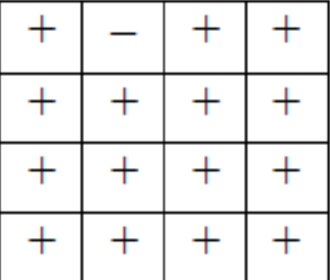
\includegraphics[width=0.2\linewidth]{task1.png}
		\end{figure}
	\end{center}
	\vspace{-6ex}
	\task{3}100 фишек выставлены в ряд. Разрешено менять местами две фишки, стоящие через одну фишку.
	Можно ли с помощью таких операций переставить все фишки в обратном порядке?\\
	
	\task{4}Можно ли из 13 кирпичей 1×1×2 сложить куб 3×3×3 с дыркой 1×1×1 в центре?
	
	
	\task{5} Все поля шахматной доски 8×8 покрыли 32 косточками домино (каждая косточка закрывает в точности два поля).
	Докажите, что число вертикально лежащих косточек чётно.\\
	\task{6}В шахматном турнире участвовали семь школьников. Известно, что
	Миша сыграл 6 партий, Коля – 5, Илья и Гриша – по три, Андрей и Сева – по
	две, а Максим – одну. С кем сыграл Илья?\\
	\task{7}За столом сидит 5 мальчиков и 7 девочек, а на столе в вазе лежат   конфеты. Некоторые из детей знакомы. Каждая девочка дала по конфете из вазы знакомому мальчику, а затем каждый мальчик дал по конфете из вазы незнакомой девочке. После этого в вазе не осталось конфет. Сколько конфет было в вазе?\\
	\task{8}Джон, приехав из Диснейленда, рассказывал, что там на заколдованном озере имеются семь островов, с каждого из которых ведет один, три или пять мостов. Верно ли, что хотя бы один из этих мостов обязательно выходит на берег озера?\\
	\task{9}Можно ли нарисовать на плоскости 15 окружностей так, чтобы одна пересекалась ровно с одной из оставшихся,
	две — ровно с двумя, три — ровно с тремя, четыре — ровно с четырьмя и пять — ровно с пятью из оставшихся окружностей?\\
	\task{10} На доску 8×8 уложен 21 прямоугольник  3×1 какая клетка могла остаться незакрытой?\\
	\task{11} Можно ли нарисовать на плоскости 15 окружностей так, чтобы одна пересекалась ровно с одной из оставшихся,
	две — ровно с двумя, три — ровно с тремя, четыре — ровно с четырьмя и пять — ровно с пятью из оставшихся окружностей?\\
	\task{12}Пете подарили набор "Юный паркетчик", состоящий из 12 триминошек
	Хулиган Вася заменил одну из них на уголок
	. Сможет ли Петя сложить квадрат
	6×6?\\
	\task{13} На доске 10×10 для "морского боя" стоит 4-палубный корабль. Какое наименьшее
	число выстрелов необходимо сделать, чтобы наверняка ранить его?\\
\end{document} 